\documentclass[a4paper,11pt]{article}

\usepackage[english]{babel}
\usepackage[utf8]{inputenc}
\usepackage[vmargin=3.5cm,hmargin=2cm]{geometry}
\usepackage{graphicx}
\usepackage{caption}
\usepackage{subcaption}
\usepackage{amsmath}
\usepackage{mathtools}
\usepackage{fancyhdr}
\usepackage{listings}

\setlength{\footskip}{0cm}
\setlength\parindent{0pt}
\addtolength{\footskip}{0.8cm}
\addtolength{\headsep}{-.5cm}

\title{\bfseries Lab 4.1: \\ Linear Modulation over a Noiseless Ideal Channel\\}
\date{}

\lfoot{}
\cfoot{}
\rfoot{\textbf{Communication Systems} \\ Teresa Algarra Ulierte }

\renewcommand{\headrulewidth}{0.5pt}
\renewcommand{\footrulewidth}{0.5pt}

\begin{document}
\renewcommand\contentsname{\vspace{-1cm}}
\maketitle
\lstset{language=Matlab}

\begin{centering}
    Teresa Algarra Ulierte \\
    Student ID: teresaalgarraulierte \\
    Perm number: 7626872 \\
\end{centering}

\vspace{3cm}

\begin{figure}[!ht]
	\centering
	
\includegraphics[scale = 5]{images/portada.jpeg}
\end{figure}

\newpage

\section{Goal of the lab:}

This is the first of a sequence of software labs which gradually develop a
reasonably complete Matlab simulator for a linearly modulated system. The
follow-on labs are Software Lab 6.1 in Chapter 6, and Software Lab 8.1 in
Chapter 8. In this lab I worked with upsampling and linear modulation filters to
measure and analyze the resulting data.

\section{Laboratory assignment:}

First of all, I wrote a MatLab funtion  analogous to Code Fragment 4.B.1 to
generate a SRRC pulse. The function gives back the SRRC pulse and the time
vector associated with it given three inputs: the excess bandwidth, the sampling
rate and over how many periods it should be calculated.

\bigskip

\begin{lstlisting}

  function [rc,time_axis] = srrc_pulse(a,m,l)

      length_os = floor(l*m);                     %Number of samples
      z = cumsum(ones(length_os,1))/m;            %Time vector
      N1 = 4*a*cos(pi*(1+a)*z);                   %Numerator Term 1
      N2 = pi*(1-a)*sinc((1-a)*z);                %Numerator Term 2
      D = (pi.*(1-16.*a.^2.*z.^2));               %Denominator
      zerotest = m/(4*a);                         %Location of zeros
      n = 1/4/a + 1e-7;                           %Value for the zeros
      if (zerotest == floor(zerotest))            %Zeros loop
          N1(zerotest) = 4*a*cos(pi*(1+a)*n);     %Numerator Term 1
          N2(zerotest) = pi*(1-a)*sinc((1-a)*n);  %Numerator Term 2
          D(zerotest) = (pi.*(1-16.*a.^2.*n.^2)); %Denominator
      end                                         %End of the loop
      G = (N1+N2)./D;                             %One side of peak
      rc = [flipud(G);1;G];                       %Peak reflection
      time_axis = [flipud(-z);0;z];               %Time vector

  end

\end{lstlisting}

\bigskip

I set the denominator zeros in $\frac{m}{4a}$, and defined the function for
those zero values.

\newpage

For an excess bandwidth of 22%, a sampling rate of $4/T$ and an interval of
$[-5T, 5T]$, the resulting plot was:

\begin{figure}[!hp]
    \begin{center}
      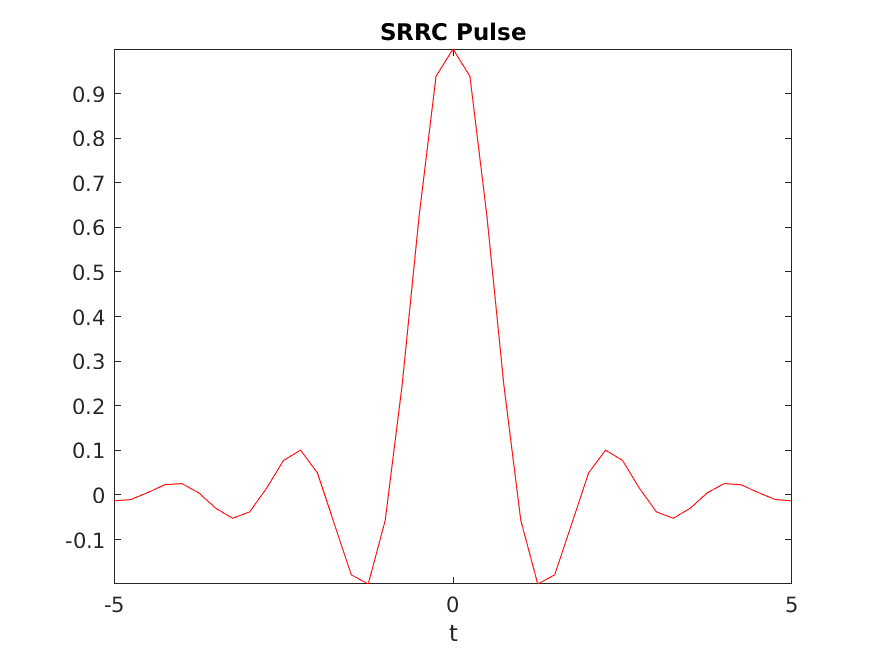
\includegraphics[width=0.6\textwidth]{images/exercise1.png}
      \captionof{figure}{SRRC}
    \end{center}
\end{figure}

For exercise 2 I used the \textbf{contFT} function created for previous labs
to compute the Fourier Transform of out SRRC pulse. The resulting plot was:

\begin{figure}[!hp]
    \begin{center}
      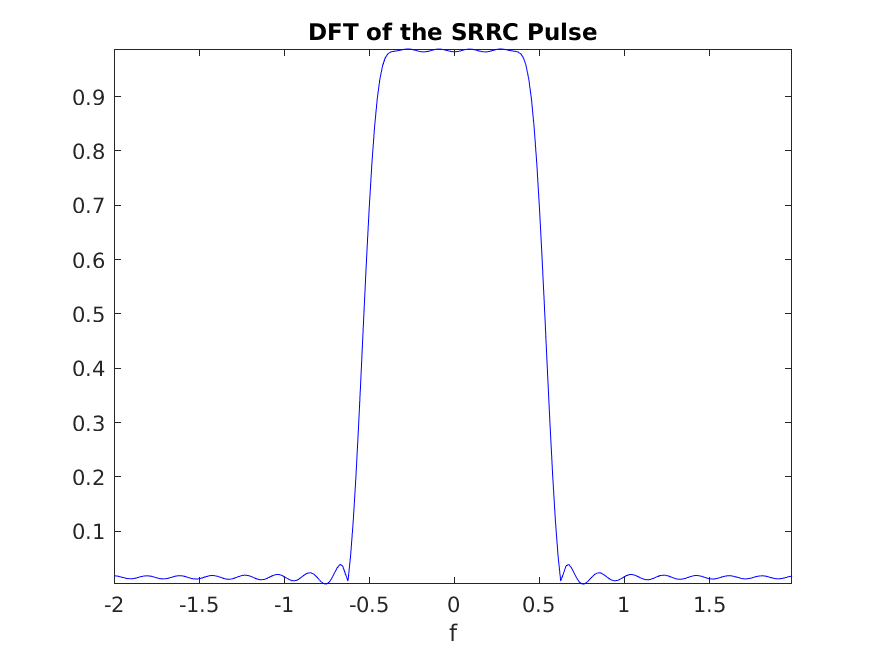
\includegraphics[width=0.6\textwidth]{images/exercise2.png}
      \captionof{figure}{$\mathcal{F}(SRRC)$}
    \end{center}
\end{figure}

\newpage

I generated 100 random bits taking values in $\{0, 1\}$ with the function
\textbf{randi}, and mapped them to symbols $b[n]$ taking values in $\{-1, +1\}$,
with 0 mapped to +1 and 1 to -1 with an \textbf{if} loop inside a \textbf{for}
loop.

\bigskip

\begin{lstlisting}

  for i = 1:100                             %Loop size
    if a(i) == 0                            %Mapping 0s to 1s
        b(i) = 1;                           %Mapping 0s to 1s
    elseif a(i) == 1                        %Mapping 1s to -1s
        b(i) = -1;                          %Mapping 1s to -1s
    end                                     %End of conditions
  end                                       %End of loop

\end{lstlisting}

\bigskip

The result was:

\begin{figure}[!hp]
    \begin{center}
      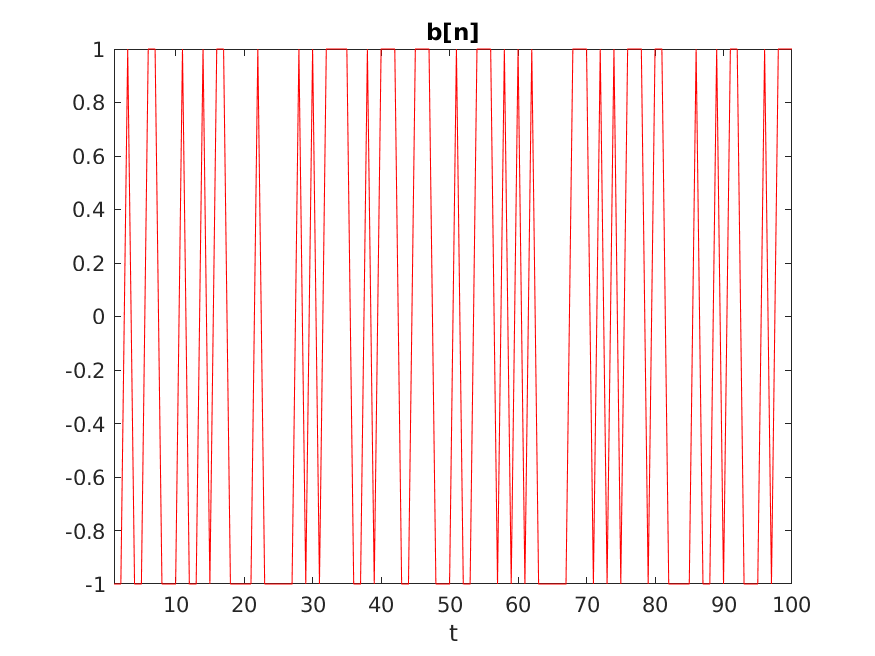
\includegraphics[width=0.9\textwidth]{images/exercise3.png}
      \captionof{figure}{$b[n]$}
    \end{center}
\end{figure}

\newpage

Then I upsampled $b[n]$ and sent the result through the system, which I did
convolving $b[n]$ with $g(t)$ using the \textbf{conv} MatLab function.

\bigskip

\begin{lstlisting}

  ns_u = 1+(ns-1)*m;                          %Upsampling by m
  s_u = zeros(ns_u,1);                        %Upsampling by m
  s_u(1:m:ns_u)=b;                            %Upsampling by m
  tx_o = conv(s_u,g);                         %Noiseless modulated signal
  t1 = cumsum(ones(length(tx_o),1)/m)-1/m-5;  %Time vector for tx_o
  t2 = cumsum(ones(length(s_u),1)/m)-1/m;     %Time vector for s_u

\end{lstlisting}

\bigskip

The plot of the convolution is:

\begin{figure}[!hp]
    \begin{center}
      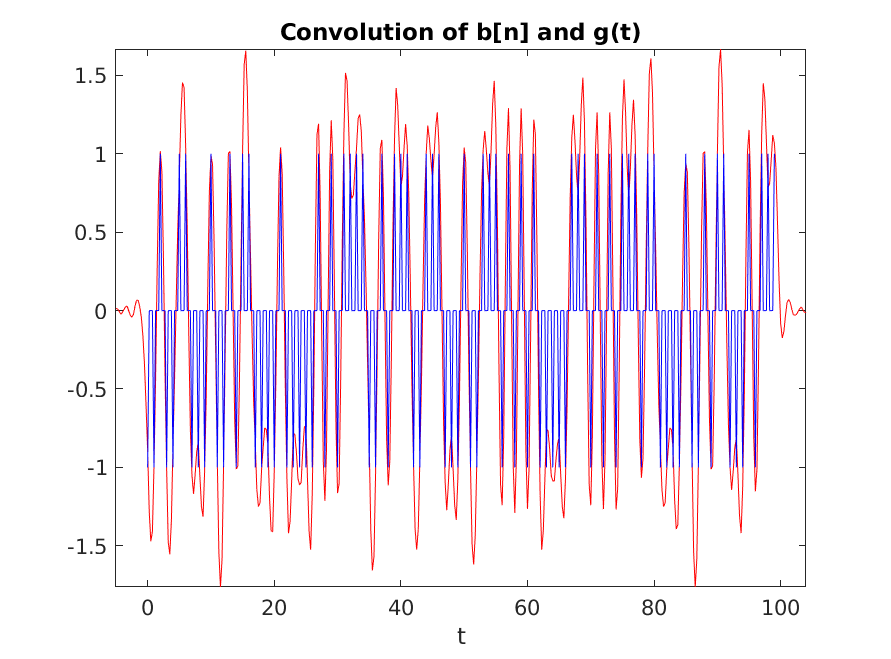
\includegraphics[width=0.9\textwidth]{images/exercise4.png}
      \captionof{figure}{$tx_o(t)$}
    \end{center}
\end{figure}

\newpage

Next, I convolved $tx_o(t)$ with $g(t)$ again, obtaining $h(t)$:

\bigskip

\begin{lstlisting}

  h = contconv(tx_o, g, 0, -5, 1/m);          %Sending b[n] through the system
  t3 = cumsum(ones(length(h),1)/m)-1/m-10;    %Time vector for tx_o
  t4 = cumsum(ones(length(s_u),1)/m)-1/m;     %Time vector for s_u

\end{lstlisting}

\bigskip

\begin{figure}[!hp]
    \begin{center}
      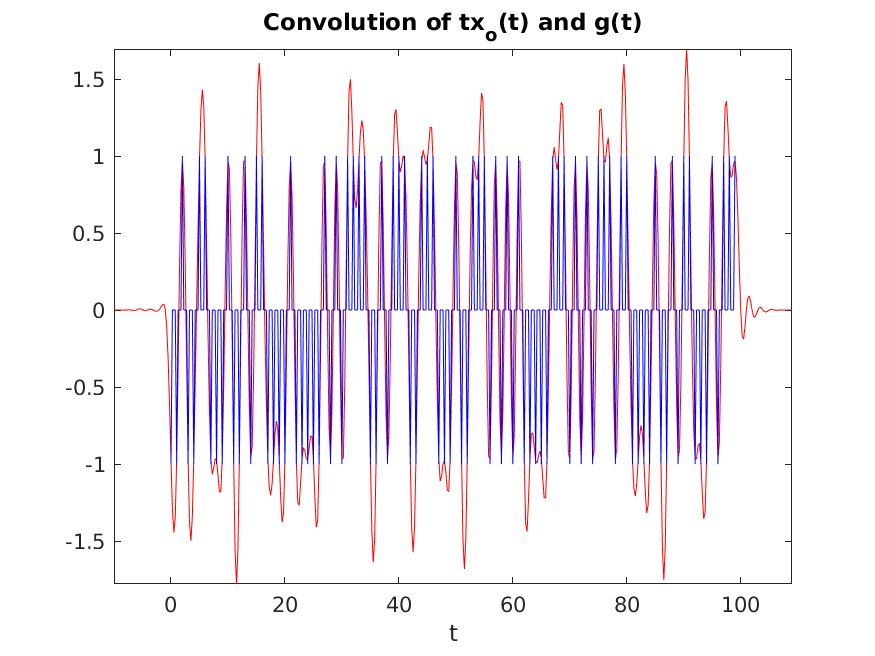
\includegraphics[width=0.9\textwidth]{images/exercise5.png}
      \captionof{figure}{$h(t)$}
    \end{center}
\end{figure}

\newpage

For exercise 6 I tried to recover the transmitted bits $a[n]$. I did so by
taking only the integers from the first zero and with a loop that did the
inverse transform of how we computed b[n].

\bigskip

\begin{lstlisting}

  t0_index = find(t1==0);                     %Looking for the first zero
  index0 = t0_index:m:m*ns+t0_index;          %Vector and steps
  r = tx_o(index0);                         	%Getting the integers only
  d = zeros(100,1);                           %Preallocating d[n]
  for i = 1:100                               %Loop size
      if r(i) < 0                             %Mapping 0s to -1s
          d(i) = 1;                           %Mapping 0s to -1s
      elseif r(i) > 0                         %Mapping 1s to 1s
          d(i) = 0;                           %Mapping 1s to 1s
      end                                     %End of conditions
  end                                         %End of loop

\end{lstlisting}

\bigskip

The result was very accurate:

\begin{figure}[!hp]
    \begin{center}
      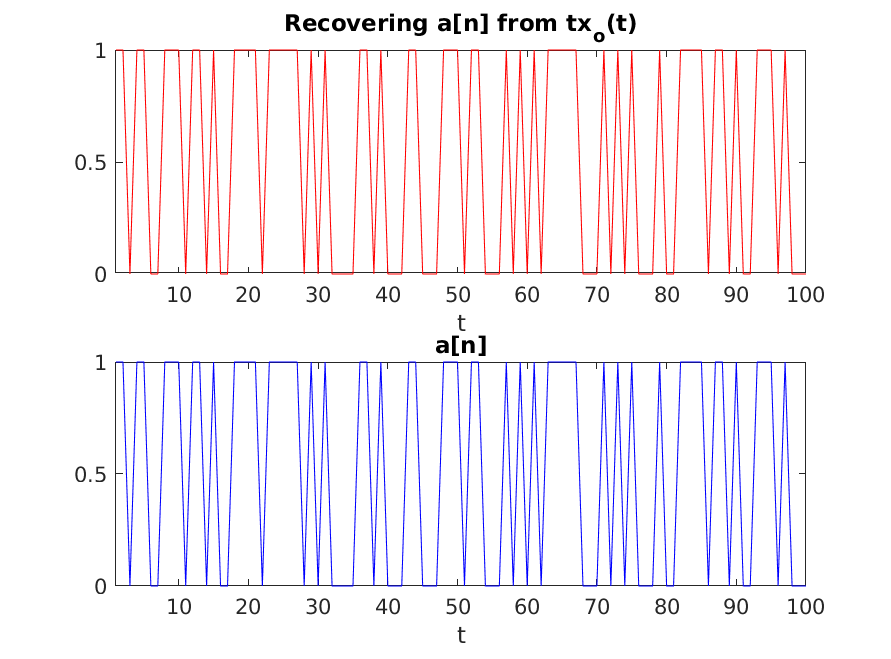
\includegraphics[width=0.9\textwidth]{images/exercise6.png}
      \captionof{figure}{Exercise 6}
    \end{center}
\end{figure}

Therefore, the error I got was 0\%.

\newpage

For exercise 7 I also tried to recover the transmitted bits $a[n]$. I copied
the code from exercise 6, so the code and the final plot were:

\bigskip

\begin{lstlisting}

  t1_index = find(t3==0);                     %Looking for the first zero
  index1 = t1_index:m:m*ns+t1_index;          %Vector and steps
  y = h(index1);                              %Getting the integers only
  f = zeros(100,1);                           %Preallocating d[n]
  for i = 1:100                               %Loop size
      if y(i) < 0                             %Mapping 0s to -1s
          f(i) = 1;                           %Mapping 0s to -1s
      elseif y(i) > 0                         %Mapping 1s to 1s
          f(i) = 0;                           %Mapping 1s to 1s
      end                                     %End of conditions
  end                                         %End of loop

\end{lstlisting}

\bigskip

\begin{figure}[!hp]
    \begin{center}
      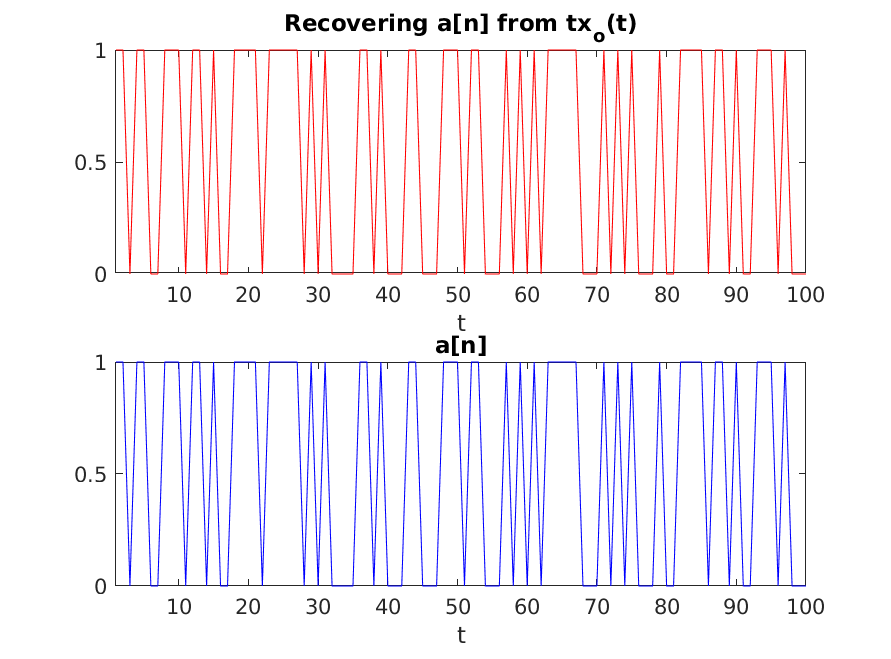
\includegraphics[width=0.9\textwidth]{images/exercise7.png}
      \captionof{figure}{Exercise 7}
    \end{center}
\end{figure}

Again, the resulting error was 0\%.

\newpage

For exercise 8, I introduced a phase offset in the receiver. Therefore, the
modeled signal was:

\begin{center}
  $tx_o e^{-j(\pi 2\Delta f t + \displaystyle\frac{\pi}{2})}$
\end{center}

\begin{lstlisting}

  df = 1/40;                                  %Given phase offset
  u = tx_o.*exp(-1j*(pi*2*df.*t1+pi/2));      %Getting the phase offset
  w = conv(u, g)/m;                           %Convolution with the filter
  t2_index = find(t3==0);                     %Looking for the first zero
  index2 = t2_index:m:m*ns+t2_index-1;        %Vector and steps
  w = w(index2);                              %Getting the integers only

\end{lstlisting}

\bigskip

When plotting the imaginary values versus the real values, the result is:

\begin{figure}[!hp]
    \begin{center}
      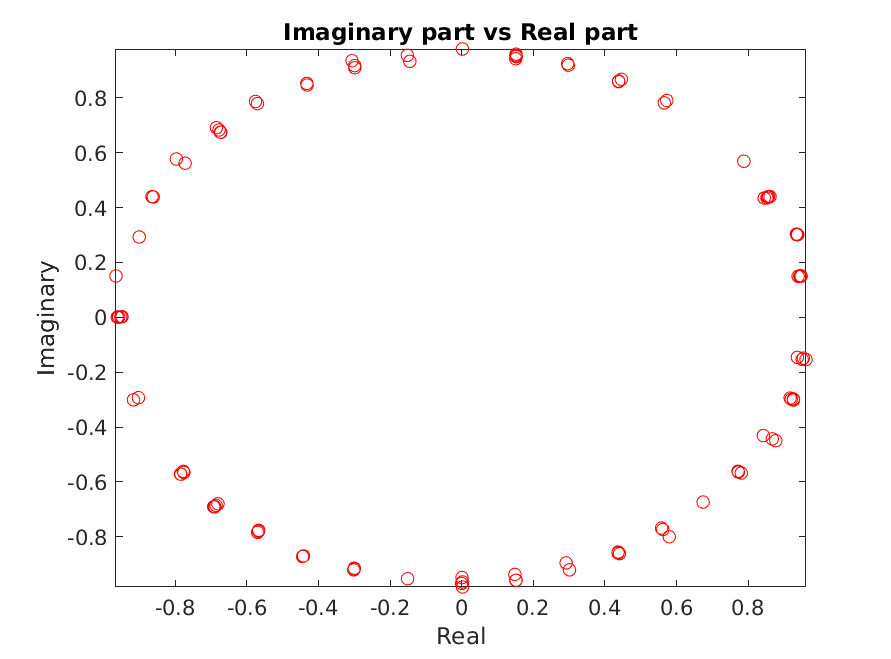
\includegraphics[width=0.9\textwidth]{images/exercise8.png}
      \captionof{figure}{Exercise 8}
    \end{center}
\end{figure}

As it can be appreciated, the plot is a circle because the phase is being
shifted all the time until coming back to the beginning.

\newpage

Lastly, for exercise 9 I took a new approach to how to recover the symbols. If

\begin{center}
  $tx_o e^{-j(\pi 2\Delta f t + \displaystyle\frac{\pi}{2})}$
\end{center}

Then when doing $w(t)w*(t-1)$ the result is $b[n]b*[n-1]$. I used this to get
back to $b[n]$ successfuly.

\bigskip

\begin{lstlisting}

  op = zeros(1,ns);                           %Preallocating the output
  op(1) = b(1);                               %Initialiting the vector
  for i=2:ns                                  %Loop
      op(i) = w(i).*conj(w(i-1)).*op(i-1);    %Output
      op(i) = sign(real(op(i)));              %Sign and real value of the output
  end                                         %End of the loop

\end{lstlisting}

\bigskip

\begin{figure}[!hp]
    \begin{center}
      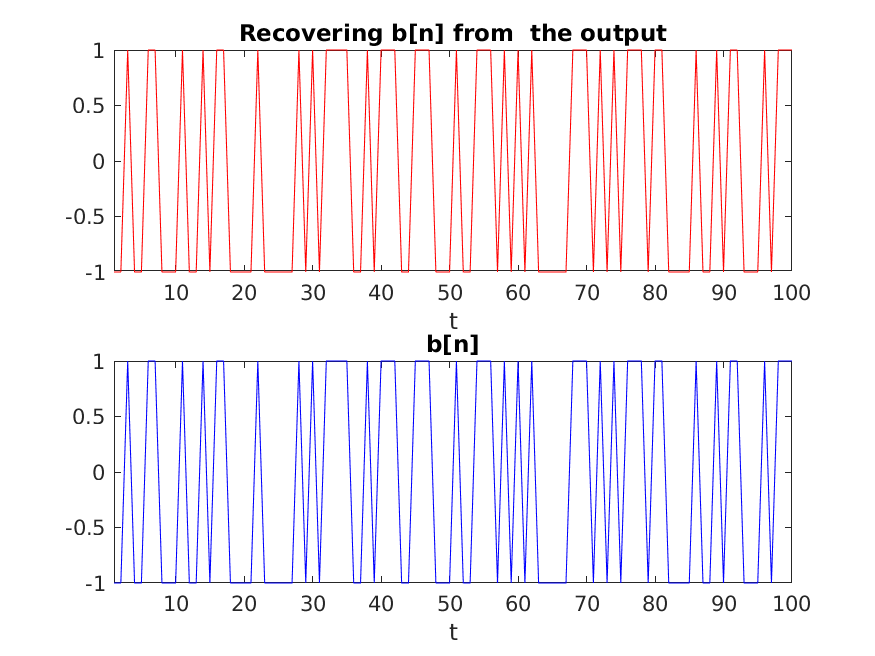
\includegraphics[width=0.9\textwidth]{images/exercise9.png}
      \captionof{figure}{Exercise 9}
    \end{center}
\end{figure}

Again, the error was 0\%.

\newpage

\section{Conclusion:}

I successfuly worked with linear modulation and got to see how BPSK functions.

There was supposed to be a different error rate for the Nyquist pulse (exercise
6) and for the non-Nyquist pulse (exercise 7). Nevertheless, maybe because of
the number of symbols taken, both error rates were 0\%. Even though, I could
see how the sampling times are crucial for the result, since it was what I had
to change the most in code.

Overall, it was a manageble lab that I got to finish fully and on time. 


\vspace{4cm}

\end{document}
